\documentclass{article}
\usepackage{amsmath, sfmath, multicol, tkz-euclide, array, enumerate, tcolorbox, tabularray}
\renewcommand{\familydefault}{\sfdefault}
\setlength{\parindent}{0cm}
\pagestyle{empty}
\usepackage[left=1in, top=0.5in, right=1in, bottom=0.5in]{geometry}
\tikzset{>=stealth}
\tcbset{colback=white}

\newcounter{example}[section]
\newenvironment{example}[1][]{\refstepcounter{example}\par\medskip
   {\color{red}\textbf{Example~\theexample. #1}}}{\medskip}

\begin{document}

\section*{Parallel Lines and Triangles}

\begin{tcolorbox}[colframe=orange!70!white, coltitle=black, title=\textbf{Today I Can}]
\begin{enumerate}
    \item Find the measures of angles of triangles.
\end{enumerate}
\end{tcolorbox}

\begin{tcolorbox}[colframe=black!20!white, opacitybacktitle=0.1, coltitle=black,  title=\textbf{Parallel Postulate}]
Given a line and a point not on the line, there is exactly one line through the point parallel to the given line.

\begin{center}
\begin{tikzpicture}[decoration={markings,
mark=at position 0.75 with {\arrow[scale=2]{>}};}, scale=0.7]
    \tkzDefPoints{0/0/A, 3/0/B, 1/1/C, 3.25/1/D}
    \tkzDrawSegment[<->, >=stealth](A,B)
    \tkzDrawPoint(C)
    \tkzDrawSegment[add = 0.35 and 0.25, <->, >=stealth, dashed](C,D)
    \tkzLabelPoint[above](C){$P$}
    \tkzLabelSegment[right,xshift=0.75in](A,B){$m$}
    \tkzMarkSegments[mark=>](A,B C,D)
\end{tikzpicture}
\end{center}
\end{tcolorbox}

\begin{tcolorbox}[colframe=black!20!white, opacitybacktitle=0.1, coltitle=black,  title=\textbf{Triangle Angle Sum}]
The angles of a triangle add up to $180^\circ$.
\end{tcolorbox}

\begin{example}
Find the values of the variables in each.

\begin{multicols}{2}
\begin{enumerate}[(a)]
\item \mbox{} \newline
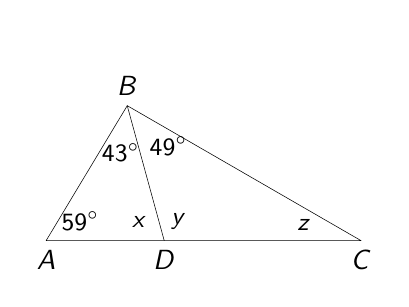
\begin{tikzpicture}
\tkzDefPoints{0/0/A, 1.5/0/D, 4/0/C}
\tkzDefShiftPoint[A](59:2){B}
\tkzDrawPolygon(A,B,C)
\tkzDrawSegment(D,B)
\tkzLabelPoints[below](A,C,D)
\tkzLabelPoints[above](B)
\tkzLabelAngle[pos=0.5](D,A,B){\small $59^\circ$}
\tkzLabelAngle[pos=-0.6](D,B,A){\small $43^\circ$}
\tkzLabelAngle[pos=-0.65,xshift=0.05in](C,B,D){\small $49^\circ$}
\tkzLabelAngle[pos=0.4](B,D,A){\small $x$}
\tkzLabelAngle[pos=0.3](C,D,B){\small $y$}
\tkzLabelAngle[pos=0.75](B,C,D){\small $z$}
\end{tikzpicture}

\item \mbox{} \newline
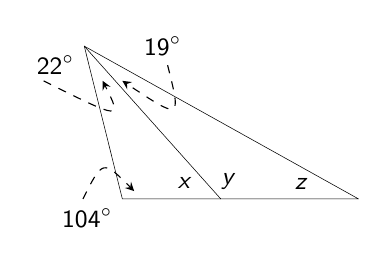
\begin{tikzpicture}
\tkzDefPoints{0/0/A, 1.25/0/B, 3/0/C}
\tkzDefShiftPoint[A](104:2){D}
\tkzDrawPolygon(A,C,D)
\tkzDrawSegment(D,B)
\node at (0,0) [anchor = north east] {\small $104^\circ$};
\draw [->, >=stealth, dashed] (-0.5, 0) .. controls (-0.25,0.5) ..  (0.15,0.1);
\node at (D) [anchor = north east] {\small $22^\circ$};
\draw [->, >=stealth, dashed] (-1, 1.5) .. controls (-0,1) .. (-0.25,1.5);
\node at (D) (hello) [anchor = west, xshift=0.25in] {\small $19^\circ$};
\draw [->, >=stealth, dashed] (hello) .. controls (0.75,1) .. (0,1.5);
\tkzLabelAngle[pos=0.5](D,B,A){\small $x$}
\tkzLabelAngle[pos=0.25](C,B,D){\small $y$}
\tkzLabelAngle[pos=0.75](D,C,B){\small $z$}
\end{tikzpicture}
\end{enumerate}
\end{multicols}
\end{example}

\vfill 

\begin{tcolorbox}[colframe=black!20!white, opacitybacktitle=0.1, coltitle=black,  title=\textbf{Exterior Angle}]
An \textbf{exterior angle} of a polygon is an angle formed by a side and an extension of an adjacent side.
\end{tcolorbox}

\begin{tcolorbox}[colframe=black!20!white, opacitybacktitle=0.1, coltitle=black,  title=\textbf{Remote Interior Angles}]
An \textbf{exterior angle} of a polygon is an angle formed by a side and an extension of an adjacent side. \newline 

\begin{minipage}{0.5\textwidth}
\begin{itemize}
    \item $\angle 1$ is an exterior angle
    \item $\angle 2$ and $\angle 3$ are remote interior angles.
\end{itemize}
\end{minipage}
\begin{minipage}{0.4\textwidth}
    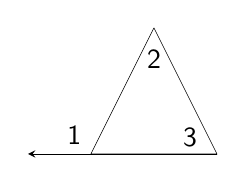
\begin{tikzpicture}[scale=0.8]
    \tkzDefPoints{0/0/A, 2/0/B, 1/2/C}
    \tkzDrawPolygon(A,B,C)
    \tkzDrawSegment[->, >=stealth, add = 0 and 0.5](B,A)
    \node at (0,0) [anchor = south east] {1};
    \tkzLabelAngle[pos=0.5](A,C,B){2}
    \tkzLabelAngle[pos=0.5](C,B,A){3}
    \end{tikzpicture}
\end{minipage}
\end{tcolorbox}

\newpage 

\begin{tcolorbox}[colframe=black!20!white, opacitybacktitle=0.1, coltitle=black,  title=\textbf{Triangle Exterior Angle Theorem}]
The measure of an exterior angle equals the sum of the measures of the remote interior angles. \newline 

\begin{minipage}{0.5\textwidth}
\begin{itemize}
    \item $m\angle 1 = m\angle 2 + m\angle 3$
\end{itemize}
\end{minipage}
\begin{minipage}{0.4\textwidth}
    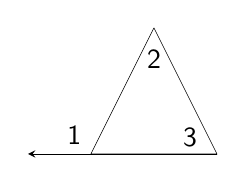
\begin{tikzpicture}[scale=0.8]
    \tkzDefPoints{0/0/A, 2/0/B, 1/2/C}
    \tkzDrawPolygon(A,B,C)
    \tkzDrawSegment[->, >=stealth, add = 0 and 0.5](B,A)
    \node at (0,0) [anchor = south east] {1};
    \tkzLabelAngle[pos=0.5](A,C,B){2}
    \tkzLabelAngle[pos=0.5](C,B,A){3}
    \end{tikzpicture}
\end{minipage}
\end{tcolorbox}

\begin{example}
Find the measure of each angle.

\begin{multicols}{2}
\begin{enumerate}[(a)]
    \item $\angle 1$  \newline

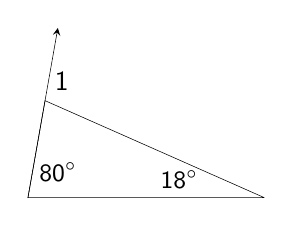
\begin{tikzpicture}
\tkzDefPoints{0/0/A, 3/0/B}
\tkzDefShiftPoint[A](80:1.25){C}
\tkzDrawPolygon(A,B,C)
\tkzDrawSegment[->, >=stealth, add = 0 and 0.75](A,C)
\tkzLabelAngle[pos=0.5](B,A,C){\small $80^\circ$}
\tkzLabelAngle[pos=1.1](C,B,A){\small $18^\circ$}
\node at (C) [anchor = south west] {1};
\end{tikzpicture}

    \item $\angle 2$  \newline

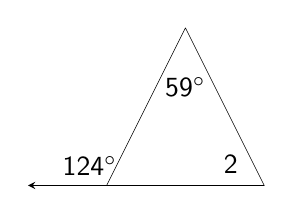
\begin{tikzpicture}
\tkzDefPoints{0/0/A, 2/0/B, 1/2/C}
\tkzDrawPolygon(A,B,C)
\tkzDrawSegment[->, >=stealth, add = 0 and 0.5](B,A)
\node at (0,0) [anchor = south east, xshift=0.1in] {$124^\circ$};
\tkzLabelAngle[pos=0.75](A,C,B){$59^\circ$}
\tkzLabelAngle[pos=0.5](C,B,A){2}
\end{tikzpicture}
\end{enumerate}
\end{multicols}
\end{example}

\vfill 

\begin{example}
Find the value of $x$. \newline 

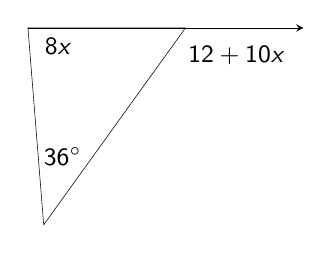
\begin{tikzpicture}
\tkzDefPoints{0/0/A, 2/0/B, 3.5/0/D, 0.2/-2.5/C}
\tkzDrawPolygon(A,B,C)
\tkzDrawSegment[->, >=stealth](A,D)
\tkzLabelAngle[pos=0.9](B,C,A){\small $36^\circ$}
\tkzLabelAngle[pos=0.35, xshift=0.05in](C,A,B){\small $8x$}
\node at (2.65,-0.35) {\small $12+10x$};
\end{tikzpicture}
\end{example}

\vfill 

\end{document}
